\subsection{YOLOv3}
\begin{frame}{}
    \LARGE Object Detection: \textbf{YOLOv3}
\end{frame}

\begin{frame}[allowframebreaks]{YOLOv3}
    \begin{figure}
        \centering
        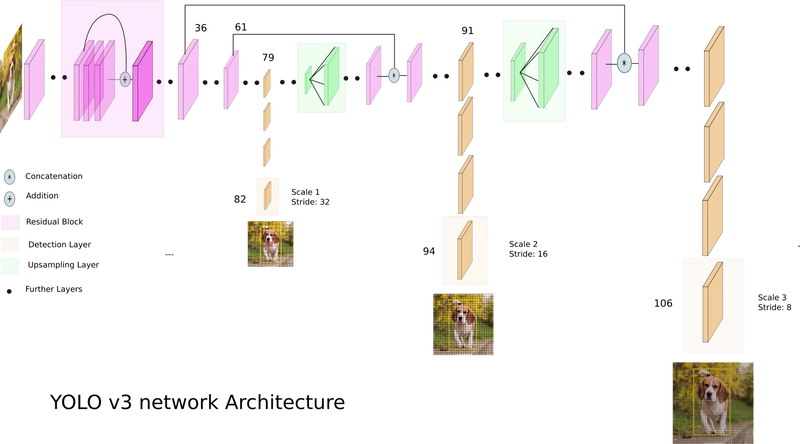
\includegraphics[width=1.0\textwidth,height=0.85\textheight,keepaspectratio]{images/object-detect/yolo-v3.png}
    \end{figure}
\framebreak
    \subsection{YOLOv4}
    \textbf{YOLOv4 (2020):} A community-driven upgrade to YOLOv3, introducing several enhancements:
    \begin{itemize}
        \item \textbf{Backbone:} CSPDarknet53 for improved feature extraction.
        \item \textbf{Activation:} Mish activation function for better non-linearity.
        \item \textbf{Neck:} Spatial Pyramid Pooling (SPP) and PANet for robust multi-scale feature aggregation.
        \item \textbf{Loss:} CIoU loss for more accurate bounding box regression.
        \item \textbf{Training Tricks:} Bag-of-Freebies and Bag-of-Specials to boost performance without increasing inference cost.
    \end{itemize}
\framebreak
    \textbf{Performance:}
    \begin{itemize}
        \item $\sim$43.5 mAP on COCO dataset.
        \item $\sim$65 FPS on GPU (real-time).
    \end{itemize}
    \textbf{Limitation:} Relies on many training and architectural tricks, making it more complex to fully understand and implement.
\end{frame}
